\documentclass{article}
\usepackage{fancyhdr}
\usepackage{ctex}
\usepackage{listings}
\usepackage{graphicx}
\usepackage[a4paper, body={18cm,22cm}]{geometry}
\usepackage{amsmath,amssymb,amstext,wasysym,enumerate,graphicx}
\usepackage{float,abstract,booktabs,indentfirst,amsmath}
\usepackage{array}
\usepackage{booktabs}
\usepackage{multirow}
\usepackage{url}
\usepackage{diagbox}
\renewcommand\arraystretch{1.4}
\usepackage{indentfirst}
\setlength{\parindent}{2em}
\usepackage{enumitem}
\setmonofont{Consolas}
\usepackage{listings}
\usepackage{xcolor}
\usepackage{makecell}
\setCJKmonofont{黑体}
\lstset{
    language = [x86masm]Assembler,
    xleftmargin = 3em,xrightmargin = 3em, aboveskip = 1em,
	backgroundcolor = \color{white}, % 背景色
	basicstyle = \small\ttfamily, % 基本样式 + 小号字体
	rulesepcolor= \color{gray}, % 代码块边框颜色
	breaklines = true, % 代码过长则换行
	numbers = left, % 行号在左侧显示
	numberstyle = \small, % 行号字体
    numbersep = -14pt, 
	keywordstyle = \color{blue!50!red!100}, % 关键字颜色
	commentstyle =\color{red!50!green!50!blue!60}, % 注释颜色
	stringstyle = \color{red}, % 字符串颜色
	frame = shadowbox, % 用(带影子效果)方框框住代码块
	showspaces = false, % 不显示空格
	columns = fixed, % 字间距固定
} 
%--------------------页眉--------------------%
\pagestyle{fancy}
\fancyhead[L]{}
\fancyhead[R]{}
\fancyhead[C]{华东师范大学软件工程学院实验报告}
\fancyfoot[C]{-\thepage-}
\renewcommand{\headrulewidth}{1.5pt}
%--------------------标题--------------------%
\begin{document}
\begin{center}
    {\Large{\textbf{\heiti 华东师范大学软件工程学院实验报告}}}
    \begin{table}[H]
        \centering
        \begin{tabular}{p{2cm}p{4cm}<{\centering}p{1cm}p{2cm}p{6cm}<{\centering}}
            姓\qquad 名: & 李鹏达 & \quad & 学\qquad 号: & 10225101460                       \\ \cline{2-2} \cline{5-5}
            实验编号:    & Lab 05 & \quad & 实验名称:    & {Writing Your Own Malloc Package}
            \\ \cline{2-2} \cline{5-5}
        \end{tabular}
    \end{table}
\end{center}
\rule{\textwidth}{1pt}
%--------------------正文--------------------%
\section{实验目的}

\begin{enumerate}[noitemsep, label={{\arabic*})}]
    \item 深入了解动态内存分配
    \item 实现一个动态内存分配器
\end{enumerate}
\normalsize
\section{实验内容与实验步骤}
\subsection{实验内容}
在本实验中,您将为 C 程序编写一个动态存储分配器,即您自己的
\texttt{malloc},\texttt{free}和\texttt{realloc}函数。我们鼓励您创造性地探索设计空间,
实施正确、高效和快速的分配器。

我们将从吞吐量(单位时间可执行次数)和空间利用率两个方面对您的分配器进行评估。

\subsubsection{隐式空闲链表}
参考课本9.9.12的内容,我们先考虑使用隐式空闲链表来实现。

首先,我们先定义在分配器编码中所需要的基本常数和宏。

其中,在第1至3行,我们定义了所使用的基本常数——字的大小\texttt{WSIZE}和双字的大小\texttt{DSIZE},以及初始空闲块的大小和扩展时堆的默认大小\texttt{CHUNKSIZE}。

在第7行中,我们使用\texttt{PACK}宏来将大小和已分配位结合起来返回一个值,用于存放在头部或者脚部中。9至10行中,我们定义了\texttt{GET}和\texttt{PUT}宏来对参数\texttt{p} 指向的字进行读取或写入。12至13行中,宏\texttt{GET\_SIZE}和\texttt{GET\_ALLOC}可以从地址\texttt{p}的头部或脚部分别返回大小和已分配位。15至16行中,宏\texttt{HDRP}和\texttt{FTRP}分别返回指向块\texttt{bp}的头部和脚部的指针。18至19行中,\texttt{NEXT\_BLKP}和\texttt{PREV\_BLKP}则分别返回指向后面的块和指向前面的块的指针。
\begin{lstlisting}[xleftmargin = 4em,xrightmargin = 4em, aboveskip = 1em, numbers = left, language = C]
    #define WSIZE 4
    #define DSIZE 8
    #define CHUNKSIZE (1 << 12)
    
    #define MAX(x, y) ((x) > (y) ? (x) : (y))
    
    #define PACK(size, alloc) ((size) | (alloc))
    
    #define GET(p) (*(unsigned int *)(p))
    #define PUT(p, val) (*(unsigned int *)(p) = (val))
    
    #define GET_SIZE(p) (GET(p) & ~0x7)
    #define GET_ALLOC(P) (GET(P) & 0x1)
    
    #define HDRP(bp) ((char *)(bp) - WSIZE)
    #define FTRP(bp) ((char *)(bp) + GET_SIZE(HDRP(bp)) - DSIZE)
    
    #define NEXT_BLKP(bp) ((char *)(bp) + GET_SIZE(((char *)(bp) - WSIZE)))
    #define PREV_BLKP(bp) ((char *)(bp) - GET_SIZE(((char *)(bp) - DSIZE)))
\end{lstlisting}

接下来,我们需要将堆初始化。

首先我们申请四个字的空间,然后对这四个字进行初始化,第一个字是不使用的填充字,后两个字是序言块,最后一个字是结尾块。然后我们创建一个初始的空闲块。

\begin{lstlisting}[xleftmargin = 4em,xrightmargin = 4em, aboveskip = 1em, numbers = left, language = C]
    int mm_init(void) {
        if ((heap_listp = mem_sbrk(4 * WSIZE)) == (void *)-1) {
            return -1;
        }
        PUT(heap_listp, 0);
        PUT(heap_listp + 1 * WSIZE, PACK(DSIZE, 1));
        PUT(heap_listp + 2 * WSIZE, PACK(DSIZE, 1));
        PUT(heap_listp + 3 * WSIZE, PACK(0, 1));
        heap_listp += 2 * WSIZE;
        if (extend_heap(CHUNKSIZE / WSIZE) == NULL) {
            return -1;
        }
        return 0;
    }
\end{lstlisting}

在初始化堆的过程中,我们使用了\texttt{extend\_heap}函数,接下来我们需要编写这个函数来增长堆。首先我们需要将字节数转化为大小的时进行一个对齐操作。然后进行分配,以及设置头部和脚部。最后的时候还要调用合并空闲块函数,将附近空闲的块进行合并,将合并后的头指针返回。

\begin{lstlisting}[xleftmargin = 4em,xrightmargin = 4em, aboveskip = 1em, numbers = left, language = C]
    static void *extend_heap(size_t words) {
        char* bp;
        size_t size;
        size = (words & 1) ? (words + 1) * WSIZE : words * WSIZE;
        if ((bp = mem_sbrk(size)) == (void *)-1) {
            return NULL;
        }
        PUT(HDRP(bp), PACK(size, 0));
        PUT(FTRP(bp), PACK(size, 0));
        PUT(HDRP(NEXT_BLKP(bp)), PACK(0, 1));
        return coalesce(bp);
    }
\end{lstlisting}

在这个过程中,我们调用了\texttt{coalesce}函数,我们接下来需要编写这个函数来完成空闲块的合并。

合并空闲块时,我们需要先获取当前块的上一个块,以及下一个块,然后对四种情况进行讨论。情况1:前后都有填充,那么不进行任何操作。情况2:前面有填充,后面没有填充,那么指针不变,将空闲块合并即可。情况3:前面有没有填充,后面有填充,那么需要将指针先前移动一个块,然后将空闲块合并。情况4:前后都没有填充,那么将指针向前移动一个块的同时,将前后空闲块进行合并。

\begin{lstlisting}[xleftmargin = 4em,xrightmargin = 3em, aboveskip = 1em, numbers = left, language = C]
    static void *coalesce(void *bp) {
        size_t prev_alloc = GET_ALLOC(FTRP(PREV_BLKP(bp)));
        size_t next_alloc = GET_ALLOC(HDRP(NEXT_BLKP(bp)));
        size_t size = GET_SIZE(HDRP(bp));
        if (prev_alloc && next_alloc) {
            return bp;
        } else if (prev_alloc && !next_alloc) {
            size += GET_SIZE(HDRP(NEXT_BLKP(bp)));
            PUT(HDRP(bp), PACK(size, 0));
            PUT(FTRP(bp), PACK(size, 0));
        } else if (!prev_alloc && next_alloc) {
            size += GET_SIZE(HDRP(PREV_BLKP(bp)));
            PUT(FTRP(bp), PACK(size, 0));
            PUT(HDRP(PREV_BLKP(bp)), PACK(size, 0));
            bp = PREV_BLKP(bp);
        } else {
            size += GET_SIZE(HDRP(NEXT_BLKP(bp))) + GET_SIZE(HDRP(PREV_BLKP(bp)));
            PUT(HDRP(PREV_BLKP(bp)), PACK(size, 0));
            PUT(FTRP(NEXT_BLKP(bp)), PACK(size, 0));
            bp = PREV_BLKP(bp);
        }
        return bp;
    }
\end{lstlisting}

同时,我们还需要一个函数\texttt{place}来实现对空闲块的分割,来提高空闲块的利用率,减少碎片的产生。如果当前空闲块的大小要比我们要分配的内容大且超过两个字,那么空闲块将被分成两部分,一部分是用来分配的,另一部分仍然是空闲的。

\begin{lstlisting}[ xleftmargin = 4em,xrightmargin = 4em, aboveskip = 1em, numbers = left, language = C]
    static void place(void *bp, size_t asize) {
        size_t size = GET_SIZE(HDRP(bp));
        if (size - asize >= 2 * DSIZE) {
            PUT(HDRP(bp), PACK(asize, 1));
            PUT(FTRP(bp), PACK(asize, 1));
            size = size - asize;
            bp = NEXT_BLKP(bp);
            PUT(HDRP(bp), PACK(size, 0));
            PUT(FTRP(bp), PACK(size, 0));
            coalesce(bp);
        } else {
            PUT(HDRP(bp), PACK(size, 1));
            PUT(FTRP(bp), PACK(size, 1));
        }
    }
\end{lstlisting}

下一步,我们来实现查找空闲块的策略。我们使用\textbf{首次适配}策略——从头往后遍历空闲链表,直至找到第一个可以放置空闲块的地方。

\begin{lstlisting}[ xleftmargin = 4em,xrightmargin = 4em, aboveskip = 1em, numbers = left, language = C]
    static void *find_fit(size_t asize) {
        for (void *bp = heap_listp; GET_SIZE(HDRP(bp)) > 0; bp = NEXT_BLKP(bp)) {
            if (!GET_ALLOC(HDRP(bp)) && GET_SIZE(HDRP(bp)) >= asize) {
                return bp;
            }
        }
        return NULL;
    }
\end{lstlisting}

然后,我们来实现\texttt{malloc}函数。我们对\texttt{size}进行非0判断,然后对\texttt{size}进行按 8 对齐舍入,接着用首次适应策略去寻找空闲块,如果存在直接存入,并返回指针,如果不存在这么大的空闲块,那么对堆进行扩展。

\begin{lstlisting}[ xleftmargin = 4em,xrightmargin = 4em, aboveskip = 1em, numbers = left, language = C]
    void *mm_malloc(size_t size) {
        size_t asize;
        size_t extendsize;
        char *bp;
        if (size == 0) {
            return NULL;
        }
        if (size < DSIZE) {
            asize = 2 * DSIZE;
        } else {
            asize = DSIZE * ((size + DSIZE + DSIZE - 1) / DSIZE);
        }
        if ((bp = find_fit(asize)) != NULL) {
            place(bp, asize);
            return bp;
        }
        extendsize = MAX(asize, CHUNKSIZE);
        if ((bp = extend_heap(extendsize / WSIZE)) == NULL) {
            return NULL;
        }
        place(bp, asize);
        return bp;
    }
\end{lstlisting}

接下来我们实现\texttt{free}函数,将一个分配块转为空闲块。这需要我们修改它的头部和脚部,然后进行前后空闲块的合并。
\begin{lstlisting}[ xleftmargin = 4em,xrightmargin = 4em, aboveskip = 1em, numbers = left, language = C]
    void mm_free(void *ptr) {
        if (ptr == NULL) {
            return;
        }
        size_t size = GET_SIZE(HDRP(ptr));
        PUT(HDRP(ptr), PACK(size, 0));
        PUT(FTRP(ptr), PACK(size, 0));
        coalesce(ptr);
    }
\end{lstlisting}

\texttt{realloc}函数则需要我们对已分配的块进行一个重新分配。可以根据原本已经写好的代码,只需要将内存分配的函数改为自己写的内存分配函数即可。

\begin{lstlisting}[ xleftmargin = 4em,xrightmargin = 4em, aboveskip = 1em, numbers = left, language = C]
    void *mm_realloc(void *ptr, size_t size) {
        void *oldptr = ptr;
        void *newptr;
        size_t copySize;
        newptr = mm_malloc(size);
        if (newptr == NULL) return NULL;
        copySize = GET_SIZE(HDRP(ptr));
        if (size < copySize) copySize = size;
        memcpy(newptr, oldptr, copySize);
        mm_free(oldptr);
        return newptr;
    }
\end{lstlisting}
\subsubsection{显式空闲链表}

一种更好的方法是将空闲块组织为某种形式的显式数据结构。因为根据定义,程序不需要一个空闲块的主体,所以实现这个数据结构的指针可以存放在这些空闲块的主体里面。例如,堆可以组织成一个\textbf{双向空闲链表},在每个空闲块中,都包含一个 \texttt{pred}(前驱)和 \texttt{succ}(后继)指针。

使用双向链表而不是隐式空闲链表,使首次适配的分配时间从块总数的线性时间减少到了空闲块数量的线性时间。

我们使用\textbf{后进先出}(LIFO)的顺序维护链表,将新释放的块放置在链表的开始处。使用 LIFO 的顺序和首次适配的放置策略,分配器会最先检查最近使用过的块。在这种情况下,释放一个块可以在常数时间内完成。如果使用了边界标记,那么合并也可以在常数时间内完成。

我们更改空闲块的结构,在其有效载荷的开始处存放其前驱和后继指针。
我们额外定义一些宏来完成其前驱和后继的读取与写入。

\begin{lstlisting}[xleftmargin = 4em,xrightmargin = 4em, aboveskip = 1em, numbers = left, language = C]
    #define GET_PREV(p) (*(unsigned int *)(p))
    #define SET_PREV(p, val) (*(unsigned int *)(p) = (val))
    #define GET_NEXT(p) (*((unsigned int *)(p) + 1))
    #define SET_NEXT(p, val) (*((unsigned int *)(p) + 1) = (val))
\end{lstlisting}

然后,我们编写函数\texttt{list\_insert}和\texttt{list\_remove}来用于链表中节点的插入与删除。我们使用后进先出的顺序维护链表,即始终在链表的头部插入节点。

\begin{lstlisting}[xleftmargin = 4em,xrightmargin = 4em, aboveskip = 1em, numbers = left, language = C]
    static void list_insert(void *bp) {
        if (bp == NULL) return;
        if (list_head == NULL) {
          list_head = bp;
          return;
        }
        SET_NEXT(bp, (list_head));
        SET_PREV(list_head, (bp));
        list_head = bp;
    }
    
    static void list_remove(void *bp) {
        if (bp == NULL || GET_ALLOC(HDRP(bp))) return;
        void* prev = GET_PREV(bp);
        void* next = GET_NEXT(bp);
        SET_PREV(bp, 0);
        SET_NEXT(bp, 0);
        if (prev == NULL && next == NULL) {
          list_head = NULL;
        } else if (prev == NULL) {
            SET_PREV(next, 0);
            list_head = next;
        } else if (next == NULL) {
            SET_NEXT(prev, 0);
        } else {
            SET_NEXT(prev, (next));
            SET_PREV(next, (prev));
        } 
    }
\end{lstlisting}

然后,我们对\texttt{coalesce}函数、\texttt{extend\_heap}函数、\texttt{place}函数和\texttt{mm\_free}函数进行修改,使其在合并、增长堆、拆分和释放时均能够维护空闲链表。

\begin{lstlisting}[xleftmargin = 4em,xrightmargin = 3em, aboveskip = 1em, numbers = left, language = C]
    static void *coalesce(void *bp) {
        size_t prev_alloc = GET_ALLOC(FTRP(PREV_BLKP(bp)));
        size_t next_alloc = GET_ALLOC(HDRP(NEXT_BLKP(bp)));
        size_t size = GET_SIZE(HDRP(bp));
        if (prev_alloc && next_alloc) {
    /****************************************************************************/
            list_insert(bp);
    /*^^^^^^^^^^^^^^^^^^^^^^^^^^^^^^^^^^^^^^^^^^^^^^^^^^^^^^^^^^^^^^^^^^^^^^^^^^*/
            return bp;
        } else if (prev_alloc && !next_alloc) {
    /****************************************************************************/
            list_remove(NEXT_BLKP(bp));
    /*^^^^^^^^^^^^^^^^^^^^^^^^^^^^^^^^^^^^^^^^^^^^^^^^^^^^^^^^^^^^^^^^^^^^^^^^^^*/
            size += GET_SIZE(HDRP(NEXT_BLKP(bp)));
            PUT(HDRP(bp), PACK(size, 0));
            PUT(FTRP(bp), PACK(size, 0));
        } else if (!prev_alloc && next_alloc) {
    /****************************************************************************/
            list_remove(PREV_BLKP(bp));
    /*^^^^^^^^^^^^^^^^^^^^^^^^^^^^^^^^^^^^^^^^^^^^^^^^^^^^^^^^^^^^^^^^^^^^^^^^^^*/
            size += GET_SIZE(HDRP(PREV_BLKP(bp)));
            PUT(FTRP(bp), PACK(size, 0));
            PUT(HDRP(PREV_BLKP(bp)), PACK(size, 0));
            bp = PREV_BLKP(bp);
        } else {
    /****************************************************************************/
            list_remove(NEXT_BLKP(bp));
            list_remove(PREV_BLKP(bp));
    /*^^^^^^^^^^^^^^^^^^^^^^^^^^^^^^^^^^^^^^^^^^^^^^^^^^^^^^^^^^^^^^^^^^^^^^^^^^*/
            size += GET_SIZE(HDRP(NEXT_BLKP(bp))) + GET_SIZE(HDRP(PREV_BLKP(bp)));
            PUT(HDRP(PREV_BLKP(bp)), PACK(size, 0));
            PUT(FTRP(NEXT_BLKP(bp)), PACK(size, 0));
            bp = PREV_BLKP(bp);
        }
    /****************************************************************************/
        list_insert(bp);
    /*^^^^^^^^^^^^^^^^^^^^^^^^^^^^^^^^^^^^^^^^^^^^^^^^^^^^^^^^^^^^^^^^^^^^^^^^^^*/
        return bp;
    }
    
    static void *extend_heap(size_t words) {
        char* bp;
        size_t size;
        size = (words & 1) ? (words + 1) * WSIZE : words * WSIZE;
        if ((bp = mem_sbrk(size)) == (void *)-1) {
            return NULL;
        }
        PUT(HDRP(bp), PACK(size, 0));
        PUT(FTRP(bp), PACK(size, 0));
    /****************************************************************************/
        SET_NEXT(bp, 0);
        SET_PREV(bp, 0);
    /*^^^^^^^^^^^^^^^^^^^^^^^^^^^^^^^^^^^^^^^^^^^^^^^^^^^^^^^^^^^^^^^^^^^^^^^^^^*/
        PUT(HDRP(NEXT_BLKP(bp)), PACK(0, 1));
        return coalesce(bp);
    }

    static void place(void *bp, size_t asize) {
        size_t size = GET_SIZE(HDRP(bp));
        list_remove(bp);
        if (size - asize >= 2 * DSIZE) {
            PUT(HDRP(bp), PACK(asize, 1));
            PUT(FTRP(bp), PACK(asize, 1));
            size = size - asize;
            bp = NEXT_BLKP(bp);
    /****************************************************************************/
            SET_NEXT(bp, 0);
            SET_PREV(bp, 0);
    /*^^^^^^^^^^^^^^^^^^^^^^^^^^^^^^^^^^^^^^^^^^^^^^^^^^^^^^^^^^^^^^^^^^^^^^^^^^*/
            PUT(HDRP(bp), PACK(size, 0));
            PUT(FTRP(bp), PACK(size, 0));
            coalesce(bp);
        } else {
            PUT(HDRP(bp), PACK(size, 1));
            PUT(FTRP(bp), PACK(size, 1));
        }
    }

    void mm_free(void *ptr) {
        if (ptr == NULL) {
            return;
        }
        size_t size = GET_SIZE(HDRP(ptr));
        PUT(HDRP(ptr), PACK(size, 0));
        PUT(FTRP(ptr), PACK(size, 0));
    /****************************************************************************/
        SET_NEXT(ptr, 0);
        SET_PREV(ptr, 0);
    /*^^^^^^^^^^^^^^^^^^^^^^^^^^^^^^^^^^^^^^^^^^^^^^^^^^^^^^^^^^^^^^^^^^^^^^^^^^*/
        coalesce(ptr);
    }
\end{lstlisting}

最后,我们重新编写\texttt{find\_fit}函数,进而实现在显式空闲链表中的查找。

\begin{lstlisting}[xleftmargin = 4em,xrightmargin = 4em, aboveskip = 1em, numbers = left, language = C]
    static void *find_fit(size_t asize) {
        for (void *bp = list_head; bp; bp = GET_NEXT(bp)) {
            if (GET_SIZE(HDRP(bp)) >= asize) {
                return bp;
            }
        }
        return NULL;
    }
\end{lstlisting}

\normalsize
\subsection{实验步骤}

\begin{enumerate}[noitemsep, label={{\arabic*})}]
    \item 解打包\texttt{malloc-handout.tar}
          \begin{lstlisting}[language=bash]
    linux> tar -xvf malloc-handout.tar
    \end{lstlisting}
    \item 阅读要求,编写\texttt{mm.c}
    \item 编译
          \begin{lstlisting}[language=bash]
    linux> make
    \end{lstlisting}
    \item 评测
          \begin{lstlisting}[language=bash]
    linux> ./mdriver -av -t traces
    \end{lstlisting}

\end{enumerate}
\normalsize
\section{实验过程与分析}

\subsection{隐式空闲链表}
实验的运行结果如下:
\begin{figure}[H]
    \centering
    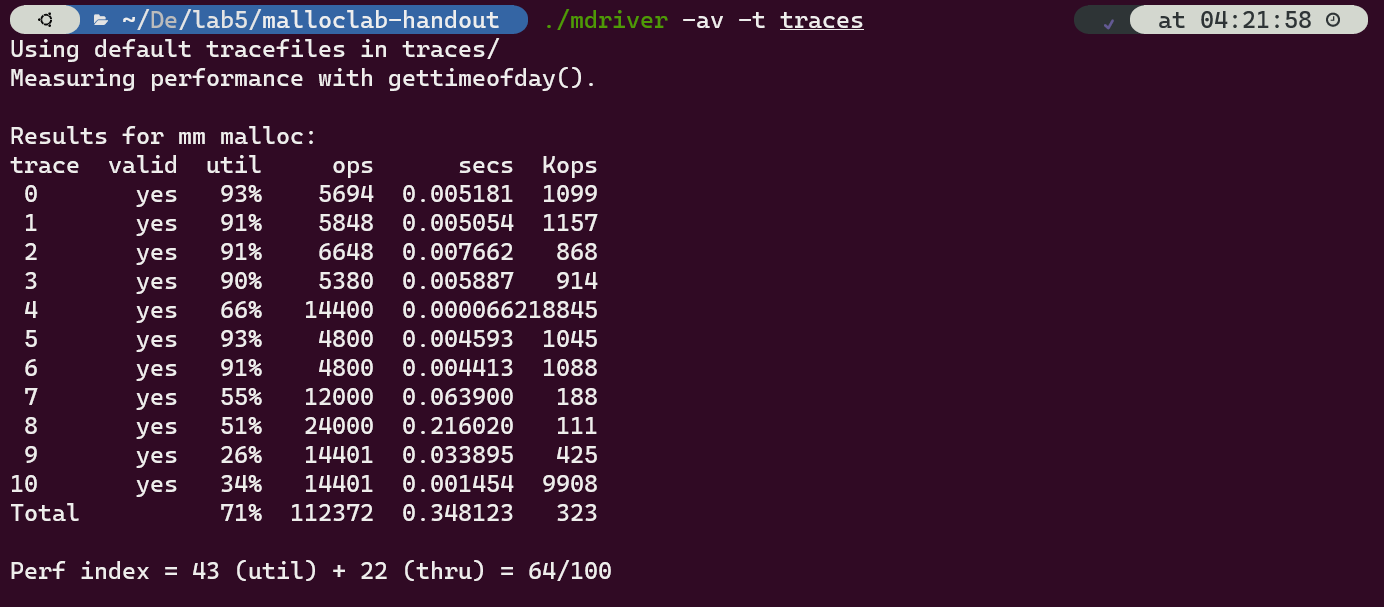
\includegraphics[width=15cm]{1.png}
    \caption{运行结果}
\end{figure}
\subsection{显式空闲链表}
实验的运行结果如下:
\begin{figure}[H]
    \centering
    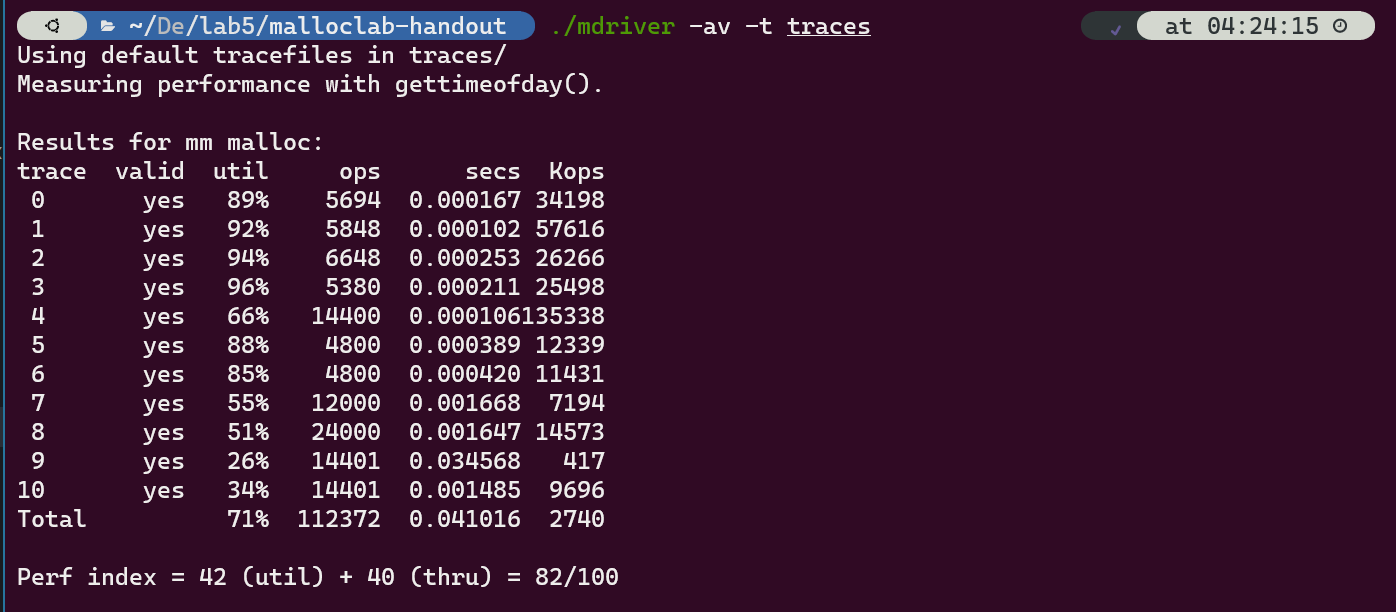
\includegraphics[width=15cm]{2.png}
    \caption{运行结果}
\end{figure}


\normalsize
\section{实验结果总结}

通过本次实验,我对 动态分配内存的内容有了一个深刻的印象,对概念的掌握更加清晰,也充分明白了该如何去利用 C 语言对分配器进行模拟,对指针的运用也有了一定的能力提升。

实验中也存在一些不足,例如可以使用分离空闲链表来进一步优化,\texttt{realloc}函数的效率也有待提高。

\normalsize

\section{附录(源代码)}

\subsection{隐式空闲链表}
\begin{lstlisting}[xleftmargin = 4em,xrightmargin = 3em, aboveskip = 1em, numbers = left, language = C]
    /*
     * mm-naive.c - The fastest, least memory-efficient malloc package.
     * 
     * In this naive approach, a block is allocated by simply incrementing
     * the brk pointer.  A block is pure payload. There are no headers or
     * footers.  Blocks are never coalesced or reused. Realloc is
     * implemented directly using mm_malloc and mm_free.
     *
     * NOTE TO STUDENTS: Replace this header comment with your own header
     * comment that gives a high level description of your solution.
     */
    #include <stdio.h>
    #include <stdlib.h>
    #include <assert.h>
    #include <unistd.h>
    #include <string.h>

    #include "mm.h"
    #include "memlib.h"

    /*********************************************************
    * NOTE TO STUDENTS: Before you do anything else, please
    * provide your team information in the following struct.
    ********************************************************/
    team_t team = {
        /* Team name */
        "team",
        /* First member's full name */
        "Pengda Li",
        /* First member's email address */
        "10225101460@stu.ecnu.edu.cn",
        /* Second member's full name (leave blank if none) */
        "",
        /* Second member's email address (leave blank if none) */
        ""
    };

    /* single word (4) or double word (8) alignment */
    #define ALIGNMENT 8

    /* rounds up to the nearest multiple of ALIGNMENT */
    #define ALIGN(size) (((size) + (ALIGNMENT-1)) & ~0x7)

    #define SIZE_T_SIZE (ALIGN(sizeof(size_t)))

    // Basic constants and macros
    #define WSIZE 4
    #define DSIZE 8
    #define CHUNKSIZE (1 << 12)

    #define MAX(x, y) ((x) > (y) ? (x) : (y))

    #define PACK(size, alloc) ((size) | (alloc))

    #define GET(p) (*(unsigned int *)(p))
    #define PUT(p, val) (*(unsigned int *)(p) = (val))

    #define GET_SIZE(p) (GET(p) & ~0x7)
    #define GET_ALLOC(P) (GET(P) & 0x1)

    #define HDRP(bp) ((char *)(bp) - WSIZE)
    #define FTRP(bp) ((char *)(bp) + GET_SIZE(HDRP(bp)) - DSIZE)

    #define NEXT_BLKP(bp) ((char *)(bp) + GET_SIZE(((char *)(bp) - WSIZE)))
    #define PREV_BLKP(bp) ((char *)(bp) - GET_SIZE(((char *)(bp) - DSIZE)))

    static char * heap_listp;

    static void *coalesce(void *bp) {
        size_t prev_alloc = GET_ALLOC(FTRP(PREV_BLKP(bp)));
        size_t next_alloc = GET_ALLOC(HDRP(NEXT_BLKP(bp)));
        size_t size = GET_SIZE(HDRP(bp));
        if (prev_alloc && next_alloc) {
            return bp;
        } else if (prev_alloc && !next_alloc) {
            size += GET_SIZE(HDRP(NEXT_BLKP(bp)));
            PUT(HDRP(bp), PACK(size, 0));
            PUT(FTRP(bp), PACK(size, 0));
        } else if (!prev_alloc && next_alloc) {
            size += GET_SIZE(HDRP(PREV_BLKP(bp)));
            PUT(FTRP(bp), PACK(size, 0));
            PUT(HDRP(PREV_BLKP(bp)), PACK(size, 0));
            bp = PREV_BLKP(bp);
        } else {
            size += GET_SIZE(HDRP(NEXT_BLKP(bp))) + GET_SIZE(HDRP(PREV_BLKP(bp)));
            PUT(HDRP(PREV_BLKP(bp)), PACK(size, 0));
            PUT(FTRP(NEXT_BLKP(bp)), PACK(size, 0));
            bp = PREV_BLKP(bp);
        }
        return bp;
    }

    static void *extend_heap(size_t words) {
        char* bp;
        size_t size;
        size = (words & 1) ? (words + 1) * WSIZE : words * WSIZE;
        if ((bp = mem_sbrk(size)) == (void *)-1) {
            return NULL;
        }
        PUT(HDRP(bp), PACK(size, 0));
        PUT(FTRP(bp), PACK(size, 0));
        PUT(HDRP(NEXT_BLKP(bp)), PACK(0, 1));
        return coalesce(bp);
    }

    static void *find_fit(size_t asize) {
        for (void *bp = heap_listp; GET_SIZE(HDRP(bp)) > 0; bp = NEXT_BLKP(bp)) {
            if (!GET_ALLOC(HDRP(bp)) && GET_SIZE(HDRP(bp)) > asize) {
                return bp;
            }
        }
        return NULL;
    }

    static void place(void *bp, size_t asize) {
        size_t size = GET_SIZE(HDRP(bp));
        if (size - asize >= 2 * DSIZE) {
            PUT(HDRP(bp), PACK(asize, 1));
            PUT(FTRP(bp), PACK(asize, 1));
            size = size - asize;
            bp = NEXT_BLKP(bp);
            PUT(HDRP(bp), PACK(size, 0));
            PUT(FTRP(bp), PACK(size, 0));
        } else {
            PUT(HDRP(bp), PACK(size, 1));
            PUT(FTRP(bp), PACK(size, 1));
        }
    }


    /* 
    * mm_init - initialize the malloc package.
    */
    int mm_init(void) {
        if ((heap_listp = mem_sbrk(4 * WSIZE)) == (void *)-1) {
            return -1;
        }
        PUT(heap_listp, 0);
        PUT(heap_listp + 1 * WSIZE, PACK(DSIZE, 1));
        PUT(heap_listp + 2 * WSIZE, PACK(DSIZE, 1));
        PUT(heap_listp + 3 * WSIZE, PACK(0, 1));
        heap_listp += 2 * WSIZE;
        if (extend_heap(CHUNKSIZE / WSIZE) == NULL) {
            return -1;
        }
        return 0;
    }

    /* 
    * mm_malloc - Allocate a block by incrementing the brk pointer.
    *     Always allocate a block whose size is a multiple of the alignment.
    */
    void *mm_malloc(size_t size) {
        size_t asize;
        size_t extendsize;
        char *bp;
        if (size == 0) {
            return NULL;
        }
        if (size < DSIZE) {
            asize = 2 * DSIZE;
        } else {
            asize = DSIZE * ((size + DSIZE + DSIZE - 1) / DSIZE);
        }
        if ((bp = find_fit(asize)) != NULL) {
            place(bp, asize);
            return bp;
        }
        extendsize = MAX(asize, CHUNKSIZE);
        if ((bp = extend_heap(extendsize / WSIZE)) == NULL) {
            return NULL;
        }
        place(bp, asize);
        return bp;
    }

    /*
    * mm_free - Freeing a block does nothing.
    */
    void mm_free(void *ptr) {
        if (ptr == NULL) {
            return;
        }
        size_t size = GET_SIZE(HDRP(ptr));
        PUT(HDRP(ptr), PACK(size, 0));
        PUT(FTRP(ptr), PACK(size, 0));
        coalesce(ptr);
    }

    /*
    * mm_realloc - Implemented simply in terms of mm_malloc and mm_free
    */
    void *mm_realloc(void *ptr, size_t size) {
        void *oldptr = ptr;
        void *newptr;
        size_t copySize;
        newptr = mm_malloc(size);
        if (newptr == NULL) return NULL;
        copySize = GET_SIZE(HDRP(ptr));
        if (size < copySize) copySize = size;
        memcpy(newptr, oldptr, copySize);
        mm_free(oldptr);
        return newptr;
    }

\end{lstlisting}
\subsection{显式空闲链表}
\begin{lstlisting}[xleftmargin = 4em,xrightmargin = 3em, aboveskip = 1em, numbers = left, language = C]
    /*
     * mm-naive.c - The fastest, least memory-efficient malloc package.
     * 
     * In this naive approach, a block is allocated by simply incrementing
     * the brk pointer.  A block is pure payload. There are no headers or
     * footers.  Blocks are never coalesced or reused. Realloc is
     * implemented directly using mm_malloc and mm_free.
     *
     * NOTE TO STUDENTS: Replace this header comment with your own header
     * comment that gives a high level description of your solution.
     */
    #include <stdio.h>
    #include <stdlib.h>
    #include <assert.h>
    #include <unistd.h>
    #include <string.h>

    #include "mm.h"
    #include "memlib.h"

    /*********************************************************
    * NOTE TO STUDENTS: Before you do anything else, please
    * provide your team information in the following struct.
    ********************************************************/
    team_t team = {
        /* Team name */
        "team",
        /* First member's full name */
        "Pengda Li",
        /* First member's email address */
        "10225101460@stu.ecnu.edu.cn",
        /* Second member's full name (leave blank if none) */
        "",
        /* Second member's email address (leave blank if none) */
        ""
    };

    /* single word (4) or double word (8) alignment */
    #define ALIGNMENT 8

    /* rounds up to the nearest multiple of ALIGNMENT */
    #define ALIGN(size) (((size) + (ALIGNMENT-1)) & ~0x7)

    #define SIZE_T_SIZE (ALIGN(sizeof(size_t)))

    // Basic constants and macros
    #define WSIZE 4
    #define DSIZE 8
    #define CHUNKSIZE (1 << 12)

    #define MAX(x, y) ((x) > (y) ? (x) : (y))

    #define PACK(size, alloc) ((size) | (alloc))

    #define GET(p) (*(unsigned int *)(p))
    #define PUT(p, val) (*(unsigned int *)(p) = (val))

    #define GET_SIZE(p) (GET(p) & ~0x7)
    #define GET_ALLOC(P) (GET(P) & 0x1)

    #define HDRP(bp) ((char *)(bp) - WSIZE)
    #define FTRP(bp) ((char *)(bp) + GET_SIZE(HDRP(bp)) - DSIZE)

    #define NEXT_BLKP(bp) ((char *)(bp) + GET_SIZE(((char *)(bp) - WSIZE)))
    #define PREV_BLKP(bp) ((char *)(bp) - GET_SIZE(((char *)(bp) - DSIZE)))

    #define GET_PREV(p) (*(unsigned int *)(p))
    #define SET_PREV(p, val) (*(unsigned int *)(p) = (val))
    #define GET_NEXT(p) (*((unsigned int *)(p) + 1))
    #define SET_NEXT(p, val) (*((unsigned int *)(p) + 1) = (val))

    static char * heap_listp;
    static char * head;

    static void list_insert(void *bp) {
        if (bp == NULL) return;
        if (head == NULL) {
            head = bp;
            return;
        }
        SET_NEXT(bp, (head));
        SET_PREV(head, (bp));
        head = bp;
    }

    static void list_remove(void *bp) {
        if (bp == NULL || GET_ALLOC(HDRP(bp))) return;
        void* prev = GET_PREV(bp);
        void* next = GET_NEXT(bp);
        SET_PREV(bp, 0);
        SET_NEXT(bp, 0);
        if (prev == NULL && next == NULL) {
            head = NULL;
        } else if (prev == NULL) {
            SET_PREV(next, 0);
            head = next;
        } else if (next == NULL) {
            SET_NEXT(prev, 0);
        } else {
            SET_NEXT(prev, (next));
            SET_PREV(next, (prev));
        } 
    }

    static void *coalesce(void *bp) {
        size_t prev_alloc = GET_ALLOC(FTRP(PREV_BLKP(bp)));
        size_t next_alloc = GET_ALLOC(HDRP(NEXT_BLKP(bp)));
        size_t size = GET_SIZE(HDRP(bp));
        if (prev_alloc && next_alloc) {
            list_insert(bp);
            return bp;
        } else if (prev_alloc && !next_alloc) {
            list_remove(NEXT_BLKP(bp));
            size += GET_SIZE(HDRP(NEXT_BLKP(bp)));
            PUT(HDRP(bp), PACK(size, 0));
            PUT(FTRP(bp), PACK(size, 0));
        } else if (!prev_alloc && next_alloc) {
            list_remove(PREV_BLKP(bp));
            size += GET_SIZE(HDRP(PREV_BLKP(bp)));
            PUT(FTRP(bp), PACK(size, 0));
            PUT(HDRP(PREV_BLKP(bp)), PACK(size, 0));
            bp = PREV_BLKP(bp);
        } else {
            list_remove(NEXT_BLKP(bp));
            list_remove(PREV_BLKP(bp));
            size += GET_SIZE(HDRP(NEXT_BLKP(bp))) + GET_SIZE(HDRP(PREV_BLKP(bp)));
            PUT(HDRP(PREV_BLKP(bp)), PACK(size, 0));
            PUT(FTRP(NEXT_BLKP(bp)), PACK(size, 0));
            bp = PREV_BLKP(bp);
        }
        list_insert(bp);
        return bp;
    }

    static void *extend_heap(size_t words) {
        char* bp;
        size_t size;
        size = (words & 1) ? (words + 1) * WSIZE : words * WSIZE;
        if ((bp = mem_sbrk(size)) == (void *)-1) {
            return NULL;
        }
        PUT(HDRP(bp), PACK(size, 0));
        PUT(FTRP(bp), PACK(size, 0));
        SET_NEXT(bp, 0);
        SET_PREV(bp, 0);
        PUT(HDRP(NEXT_BLKP(bp)), PACK(0, 1));
        return coalesce(bp);
    }

    static void *find_fit(size_t asize) {
        for (void *bp = head; bp; bp = GET_NEXT(bp)) {
            if (GET_SIZE(HDRP(bp)) >= asize) {
                return bp;
            }
        }
        return NULL;
    }

    static void place(void *bp, size_t asize) {
        size_t size = GET_SIZE(HDRP(bp));
        list_remove(bp);
        if (size - asize >= 2 * DSIZE) {
            PUT(HDRP(bp), PACK(asize, 1));
            PUT(FTRP(bp), PACK(asize, 1));
            size = size - asize;
            bp = NEXT_BLKP(bp);
            SET_NEXT(bp, 0);
            SET_PREV(bp, 0);
            PUT(HDRP(bp), PACK(size, 0));
            PUT(FTRP(bp), PACK(size, 0));
            coalesce(bp);
        } else {
            PUT(HDRP(bp), PACK(size, 1));
            PUT(FTRP(bp), PACK(size, 1));
        }
    }


    /* 
    * mm_init - initialize the malloc package.
    */
    int mm_init(void) {
        if ((heap_listp = mem_sbrk(4 * WSIZE)) == (void *)-1) {
            return -1;
        }
        head = NULL;
        PUT(heap_listp, 0);
        PUT(heap_listp + 1 * WSIZE, PACK(DSIZE, 1));
        PUT(heap_listp + 2 * WSIZE, PACK(DSIZE, 1));
        PUT(heap_listp + 3 * WSIZE, PACK(0, 1));
        heap_listp += 2 * WSIZE;
        if (extend_heap(CHUNKSIZE / WSIZE) == NULL) {
            return -1;
        }
        return 0;
    }

    /* 
    * mm_malloc - Allocate a block by incrementing the brk pointer.
    *     Always allocate a block whose size is a multiple of the alignment.
    */
    void *mm_malloc(size_t size) {
        size_t asize;
        size_t extendsize;
        char *bp;
        if (size == 0) {
            return NULL;
        }
        if (size < DSIZE) {
            asize = 2 * DSIZE;
        } else {
            asize = DSIZE * ((size + DSIZE + DSIZE - 1) / DSIZE);
        }
        if ((bp = find_fit(asize)) != NULL) {
            place(bp, asize);
            return bp;
        }
        extendsize = MAX(asize, CHUNKSIZE);
        if ((bp = extend_heap(extendsize / WSIZE)) == NULL) {
            return NULL;
        }
        place(bp, asize);
        return bp;
    }

    /*
    * mm_free - Freeing a block does nothing.
    */
    void mm_free(void *ptr) {
        if (ptr == NULL) {
            return;
        }
        size_t size = GET_SIZE(HDRP(ptr));
        PUT(HDRP(ptr), PACK(size, 0));
        PUT(FTRP(ptr), PACK(size, 0));
        SET_NEXT(ptr, 0);
        SET_PREV(ptr, 0);
        coalesce(ptr);
    }

    /*
    * mm_realloc - Implemented simply in terms of mm_malloc and mm_free
    */
    void *mm_realloc(void *ptr, size_t size) {
        void *oldptr = ptr;
        void *newptr;
        size_t copySize;
        newptr = mm_malloc(size);
        if (newptr == NULL) return NULL;
        copySize = GET_SIZE(HDRP(ptr));
        if (size < copySize) copySize = size;
        memcpy(newptr, oldptr, copySize);
        mm_free(oldptr);
        return newptr;
    }

\end{lstlisting}
\normalsize
\end{document}